\chapter{Discussion}
\thispagestyle{plain}

\label{ch:application}

This chapter presents considerations when using the problem space analysis  (PSA) algorithms described in the previous chapters.  It details some of the implicit criteria  for effective use of the algorithms, discusses the tradeoffs between using online repair and PSA, and describes other potential applications.

\section{Algorithmic Assumptions}



The effectiveness of the algorithms described in the previous chapters requires the existence of regions in the problem space with identical solutions.  Fewer regions and larger region size allow the algorithms to be more effective.  This was demonstrated through the experiments in which  TSPs with fewer cities created fewer, larger homogeneous solution regions and had better PS Map approximation.  Likewise, elevator domains with larger N values -- that is, larger blocks of floors -- tend to be more readily approximated by the algorithms.  Conversely, increasing the number of fast elevators potentially increases the number of regions, and, consistent with the results, becomes less amenable to approximation by the algorithms.

Thus, plan solution spaces have homogeneous solution regions that the algorithms attempt to exploit.  These regions could be considered a function of a problem domain's objective function, as demonstrated by the justification for SBE.  Recall that the goal of SBE is to mathematically discover boundaries between solution regions by equating the objective functions of problem instances with differing variable features.  In this way SBE discovers problem instances for which two solutions have equal utility, thus constituting a boundary between two solution regions.  

As  seen with SBE and its skeletal generation of solution region boundaries, a TSP's solution boundaries are defined by each pairwise set of unique solutions discovered by an initial sample.  Fewer unique solutions increases the number of problem instances per solution; that is, it increases the size of the solution regions.  At a given sample rate, the larger solution regions create a greater likelihood that  a random sample will include the points necessary to identify the unique solutions within the problem space.

Other problem domains, such as the elevator domain, do not have explicit objective functions, but do have problem configurations that can serve the same purpose.  Within the TSP domain, the number of fixed cities affects the number of possible unique solutions, a fraction of which are represented in the problem space as solution regions.  In the knapsack domain, the set of static items affects the number of possible unique solutions as well.  As the value of a variable item increases, it eventually supersedes a  static item, resulting in a new solution.  For example, every problem instance in which the variable item is ``worse'' than the ``worst'' static item will have a solution that includes the static item rather than the variable item.\footnote{The evaluation of ``worse'' and ``worst'' depends on the heuristic used by the solver, but one example is the ratio of weight to value.}  The problem instances for which the variable item is ``better'' than the static item will result in a distinct solution.  Each static item presents an opportunity for a new solution. Thus, increasing the number of static items that are present in the domain results in  more distinct solutions and thereby more solution regions will exist.  

In the elevator domain, the number of blocks of floors affects the number of solution regions.  In general, the number of steps for a passenger to move from its starting to final destination is a function of the floor block that contains its starting location.  If abstracted as previously described, there is potentially little difference in the solution regardless of where in the floor block the passenger starts, which itself suggests an identical solution for several starting locations.  The greater number of floor blocks thereby leads to a greater number of solution regions.

The general conclusion is that the static characteristics have a direct impact on the number of homogeneous solution regions.  This can be observed in the previous examples in which the static characteristics tend to serve as an indicator of a threshold that variable features may cross and create a distinct solution.

In order to create these homogeneous regions, the axes used in the PS Map must be chosen appropriately, such that the problem instances with similar solutions are grouped together.  In the TSP domain, indexing by the x- and y-coordinates of the variable location resulted in homogeneous regions; in the knapsack domain, indexing by the variable item's weight and value results in homogeneous regions; and in the elevator domain, indexing by the starting passengers' starting location resulted in homogeneous solution regions.  In other domains, the surface attributes may not provide a natural grouping. For example, I briefly investigated the problem space of a game, \textit{Alien Frontiers}.    This game falls in the category of worker placement, in which a player rolls at least three and sometimes up to seven dice, and may choose to place dice of meeting certain criteria in a ``docking station.''  For example, two or three of a kind is required for some docking stations; others require three dice of consecutive increasing value (e.g. 3,4,5); and others merely require a total value of greater than seven.  Particularly in the early game, a pair is a valuable roll, and my solver would generally create one class of plan for rolls containing a pair, and another for rolls not containing a pair.  In this domain, indexing by the value of the dice did not result in homogeneous regions.  Rather, a better indexing scheme in this case would have been a derived boolean attribute, indicating ``pair'' or ``not pair.''

In addition to appropriate indexing, the plans must be abstracted enough to create similar plans that can form homogeneous regions.  This is demonstrated in the elevator domain in which the raw plans were abstracted to more generic plans.  If indexing and abstraction result in homogeneous clumps, then an either an SBE approach, in which objective functions are equated, or an SVM+SBE approach could be appropriate.  If not, SSS could be a viable alternative.


\section{Tradeoff with Online Repair}
These techniques allow a system to find solutions for large numbers of similar problem instances, providing useful information in domains that do not allow for large amounts of replanning time once an incident occurs, but in which there is some time before such an incident.  However, it is worth noting that in addition to offline version online repair, a system could also choose not to replan at all.  For example, if a system determined that the utility loss of the current solution with respect to the post-event problem instance was tolerable, then it could be reasonable to continue with the current solution.  One could also consider the external costs related to a new plan that isnot explicit in the problem instance.   For example, a new plan could require more resources than the current plan, or there could be a cost in switching plans.  In this case, if the cost of the new plan is greater than the loss from the use of the suboptimal solution, then the system could be justified in not replanning.

However, assuming that the system does determine that the overall cost analysis supports replanning, then it is worth considering how best take advantage of the offline time available to prepare for online events.  Given that the sample rate determines the accuracy of the approximated map, a system would want to use the highest sample rate possible.  In the case where the system knows the expected time until a disruptive event occurs, then this technique could be used as a contract algorithm \citep{Zilberstein99real-timeproblem-solving} -- an algorithm that is given a specific amount of time with which to find a solution -- with a sample rate:
\begin{equation*}
rate = \frac{time_{\mbox{\itshape offline}}}{time_{inst}*n_{inst}} ,
\label{eq:tradeoff}
%\caption{Relationship between sample rate and offline planning time.  $time_{offline}$ is offline planning time, $time_{inst}$ is time required to solve a problem instance, and $n_{inst}$ is the number of problem instance in the problem space.}
\end{equation*}

\noindent
where $time_{\mbox{\itshape offline}}$ is the estimated time preceding the disruptive event, $time_{inst}$ is the time required to solve a single problem instance, and $n_{inst}$ is the total number of problem instances in the space.  (More intuitively, it is the amount of offline time divided by the amount of time that would be required to solve every problem instance.) In the case where there is no knowledge of the length of time until the disruptive event, then the system can define  $time_{\mbox{\itshape offline}}$ as a periodic ``refresh'' interval that triggers the generation of a new PS Map, or use a real-time algorithm approach in which PS Maps are generated with successively larger sample rates until the time of the event.

Considering the test domains of the previous chapter, the tradeoff can be made more concrete.  The typical time to solve a 100-city TSP with the heuristic solver is three seconds on a laptop and  approximately 0.4 seconds on a high-performance machine.  The knapsack problem required .016 seconds on a high-performance machine, and the elevator domain required 30-60 seconds on the same machine.  Knowing that the online repair for a 100-city TSP has a fractional utility loss of approximately .02 and mapping that to a SVM+SBE approximation sample rate of .002 in Figure \ref{fig:100tsp_baseline}, one can insert these values to the equation.

\begin{equation*}
.002 = \frac{time_{\mbox{\itshape offline}}}{0.4sec * 10000}
\end{equation*}

This results in a $time_{\mbox{\itshape offline}}$ of eight seconds.  Thus, if the system comparable to the laptop's capability has eight seconds or more with which to preplan, then it is advantageous to use PSA.  Otherwise, plan repair is probably a better option.  For the knapsack domain, using the online repair results from Figure \ref{fig:svmsbe_knapsack_4d_baseline}, I obtain the equation

\begin{equation*}
.006 = \frac{time_{\mbox{\itshape offline}}}{.016sec * 10000}
\end{equation*}

This results in a $time_{\mbox{\itshape offline}}$ of 0.96 seconds.  Of course, determining whether investing the required lead time or the online repair time is preferable would be application-specific.  Figures \ref{fig:timing-tsp} and \ref{fig:timing-k} show the quickly increasing solver time required as the problem sizes grow larger, which would imply that the time required to generate a PS Map would also increase.  In the same way, online repair time for increasing problem complexity would also increase.  This again points to a tradeoff between the increasing solution time needed for PSA and the expected decline in the performance of online repair.

A more comprehensive view of this tradeoff is shown in Figures \ref{fig:timing-k-2d-sc} through \ref{fig:timing-k-2d-svmsbe}.  Looking at the knapsack results, there does not seem to be an especially strong correlation between the computation time and the utility loss.  Given the random nature of the SC algorithm, it is not surprising that there is a lot of variation in the results.  The other algorithms show a stronger relationship between computation time and performance.  This is not surprising given the more directed nature of these algorithms.  






\begin{figure}
\begin{center}
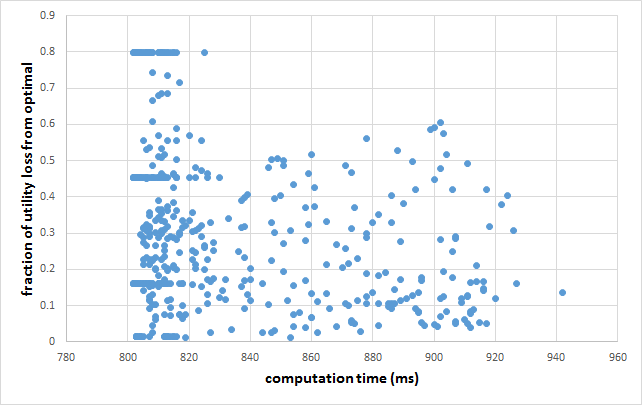
\includegraphics[scale=0.75]{pics/timing-k-2d-sc.eps}
\caption{Relationship between SC approximation computation time and map quality for a two-dimensional knapsack domain.}
\label{fig:timing-k-2d-sc}
\end{center}
\end{figure}


\begin{figure}
\begin{center}
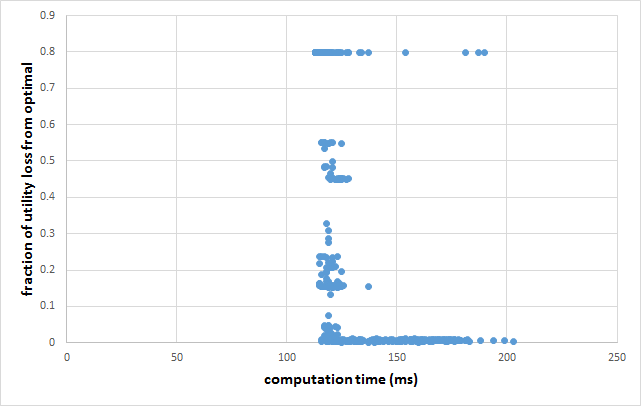
\includegraphics[scale=0.75]{pics/timing-k-2d-al.eps}
\caption{Relationship between SC+AL approximation computation time and map quality for a two-dimensional knapsack domain.}
\label{fig:timing-k-2d-al}
\end{center}
\end{figure}

\begin{figure}
\begin{center}
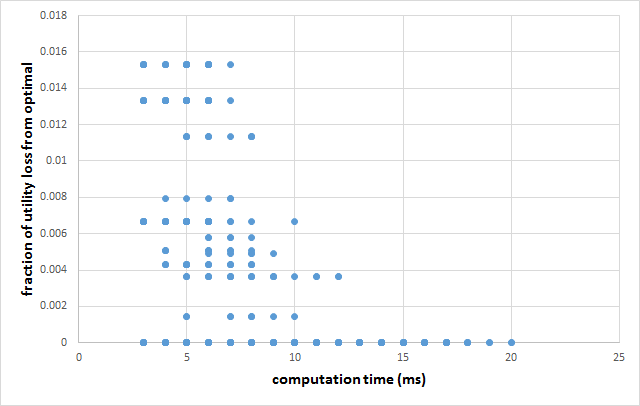
\includegraphics[scale=0.75]{pics/timing-k-2d-sss.eps}
\caption{Relationship between SSS approximation computation time and map quality for a two-dimensional knapsack domain.}
\label{fig:timing-k-2d-sss}
\end{center}
\end{figure}


\begin{figure}
\begin{center}
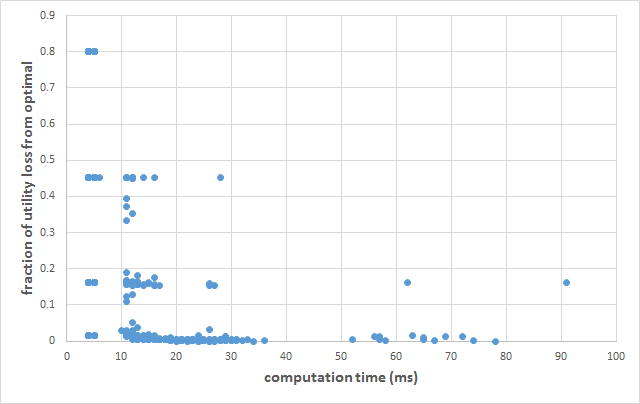
\includegraphics[scale=0.75]{pics/timing-k-2d-svm.eps}
\caption{Relationship between SVM approximation computation time and map quality for a two-dimensional knapsack domain.}
\label{fig:timing-k-2d-svm}
\end{center}
\end{figure}

\begin{figure}
\begin{center}
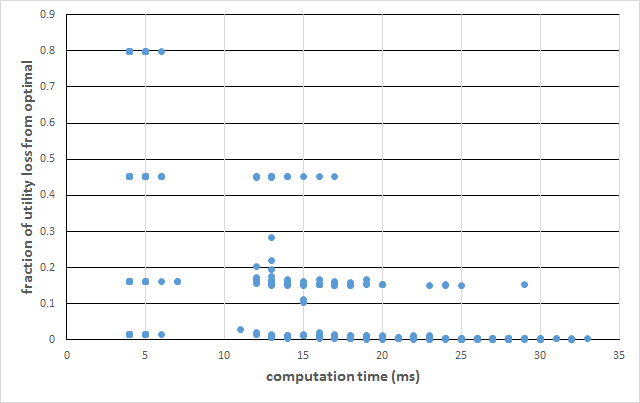
\includegraphics[scale=0.75]{pics/timing-k-2d-svmsbe.eps}
\caption{Relationship between SVM+SBE approximation computation time and map quality for a two-dimensional knapsack domain.}
\label{fig:timing-k-2d-svmsbe}
\end{center}
\end{figure}

Similar to the knapsack problem,  the elevator domain shows a strong correlation between computation time and utility loss when the more sophisticated algorithms are employed, as shown in Figures \ref{fig:timing-elevator6pass-sc} through \ref{fig:timing-elevator6pass-svmsbe}.  However, even the random SC algorithm in this domain seems to show a tendency towards better performance at high sample rates.












It is worth noting the discrete characteristic of several of the maps.  This results from very low variance in utility loss as a function of the discovered solutions.  That is, the set of solutions that the initial sampling discovers tends to determine the overall performance of the approximation algorithm.  This is most evident in the SSS algorithm, in which the assignment of the solutions to unsolved problem instances is most directly determined by the set of discovered solutions.  Recall that in SSS, each unsolved problem is assigned a solution by testing each previously discovered solution.  Other approximation algorithms attempt to avoid testing all discovered  the solutions, but, outside of SC, these algorithms still tend to use the information from the set of discovered solutions in a consistent, although not deterministic, manner.

A similar effect explains the horizontal clustering apparent in several of the maps.  This clustering is a function of low number of solutions in the space, leading to low numbers of permutations of discovered solutions during the initial sampling stage.  Again, the performance of the algorithms is sensitive to the solutions discovered.  Thus the same permutation tends to lead to similar performance of the algorithm, resulting in clustering at a specific utility loss measure.


This discrete characteristic and cluster effect appears less frequently in the elevator domain, likely due to the larger number of solutions available in the domain.  Thus, the set of discovered solutions  is more varied.




\begin{figure}
\begin{center}
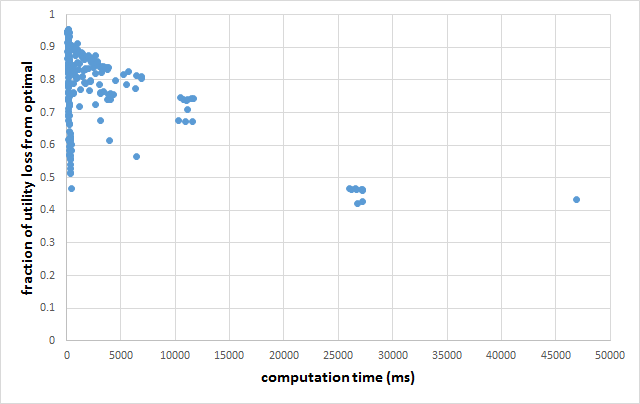
\includegraphics[scale=0.75]{pics/timing-elevator6pass-sc.eps}
\caption{Relationship between SC approximation computation time and map quality for a three-dimensional elevator domain.}
\label{fig:timing-elevator6pass-sc}
\end{center}
\end{figure}

\begin{figure}
\begin{center}
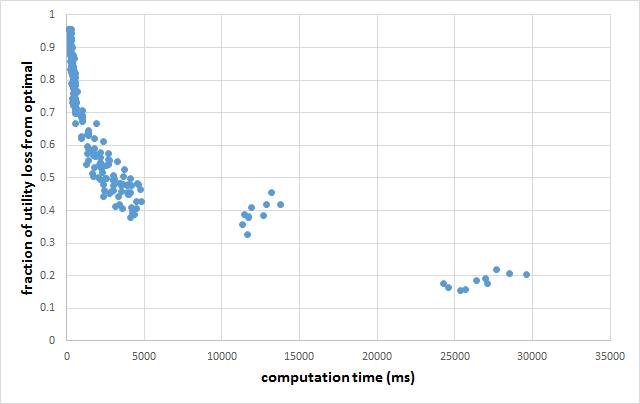
\includegraphics[scale=0.75]{pics/timing-elevator6pass-al.eps}
\caption{Relationship between SC+AL approximation computation time and map quality for a three-dimensional elevator domain.}
\label{fig:timing-elevator6pass-al}
\end{center}
\end{figure}

\begin{figure}
\begin{center}
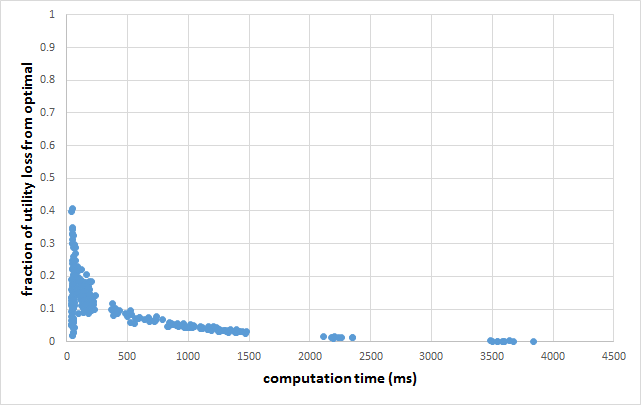
\includegraphics[scale=0.75]{pics/timing-elevator6pass-sss.eps}
\caption{Relationship between SSS approximation computation time and map quality for a three-dimensional elevator domain.}
\label{fig:timing-elevator6pass-sss}
\end{center}
\end{figure}

\begin{figure}
\begin{center}
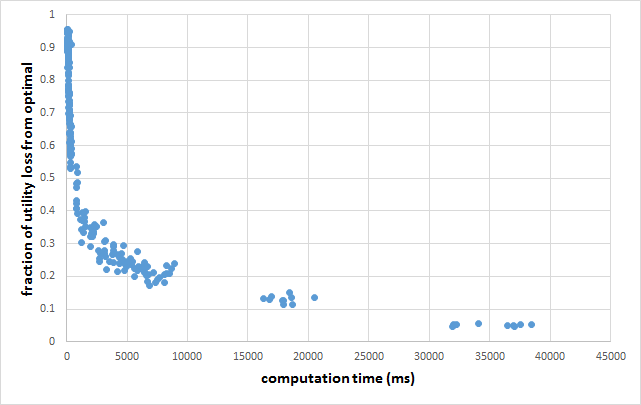
\includegraphics[scale=0.75]{pics/timing-elevator6pass-svm.eps}
\caption{Relationship between SVM approximation computation time and map quality for a three-dimensional elevator domain.}
\label{fig:timing-elevator6pass-svm}
\end{center}
\end{figure}

\begin{figure}
\begin{center}
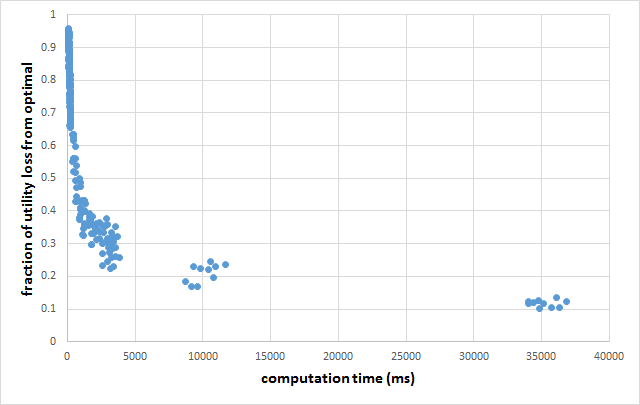
\includegraphics[scale=0.75]{pics/timing-elevator6pass-svmsbe.eps}
\caption{Relationship between SVM+SBE approximation computation time and map quality for a three-dimensional elevator domain.}
\label{fig:timing-elevator6pass-svmsbe}
\end{center}
\end{figure}

%For the elevator domain, I revisit Figure \ref{fig:svmsbe_elevator_12} and assume the best-case online repair fractional utility loss of .065.

This leaves the question of how to accurately estimate the expected performance is for a particular sample rate. Recalling that the effectiveness of the algorithms appears to be a function of the number of size of homogeneous solution regions, it may be possible to estimate the number of homogeneous solution regions by examining the  characteristics of the objective function or the problem configuration.  For example, an elevator domain with configuration M=12, N=6, with one slow elevator per block, has approximately two solution regions:  one in which the elevator in the first block picks up the passenger, and one in which the elevator in the second block picks up the passenger.  One might then speculate that the  number of solution regions is approximately $\frac{M}{N}$, assuming one slow elevator per block and zero fast elevators.  Determining the number of solution regions in other domains is potentially less straightforward.  For example, Figure \ref{fig:five_city_tsps} shows PS Maps for several randomly configured DTSPs.  The unique solutions vary from eight to eleven.


% description of number of unqiue item weights versus number of unique solutions experiment
As one experiment shows, the number of unique solutions in a knapsack PS Map is approximated by the number of unique item weights in the knapsack prior to the consideration of the variable item.  In the first experiment, I started with a knapsack of static items and generated a PS Map for several weight threshold values.  For each weight threshold, I found the knapsack solution and recorded the number of unique item weights.  I then introduced the variable item, generated the PS Map, and recorded the number of unique solutions.

In the second experiment, I kept the weight threshold constant and generated a PS Map for several static item  configurations.  As in the first experiment, I recorded the number of unique weight values in the static item set, added the variable item, generated the PS Map, then recorded the number of unique solutions in the PS Map.

The results of the first experiment demonstrate that the number of unique solutions per number of unique weights is approximately 1.02.




\begin{figure}
\begin{center}
\includegraphics[scale=0.25]{pics/FiveCityFourFixed_0-3.dat.eps}
\caption{Various high-quality PS Maps of five-city TSPs.  Total number of unique solutions varies from eight to eleven.}
\label{fig:five_city_tsps}
\end{center}
\end{figure}


\begin{figure}
\begin{center}
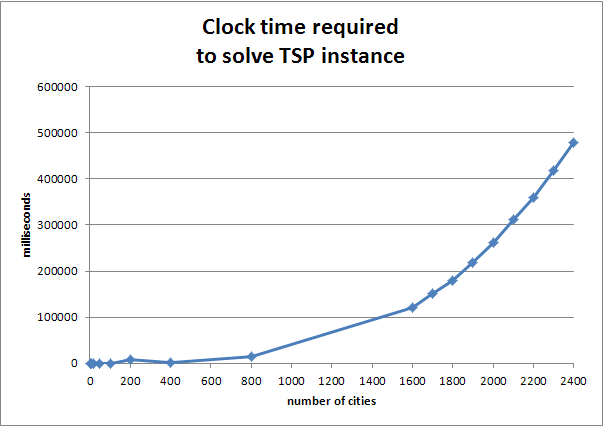
\includegraphics[scale=0.5]{pics/timing-tsp.eps}
\caption{Time required to solve TSP problems of various sizes.  The average time to solve 400-city TSPs is less that required to solve 200-city TSPs.}
\label{fig:timing-tsp}
\end{center}
\end{figure}

\begin{figure}
\begin{center}
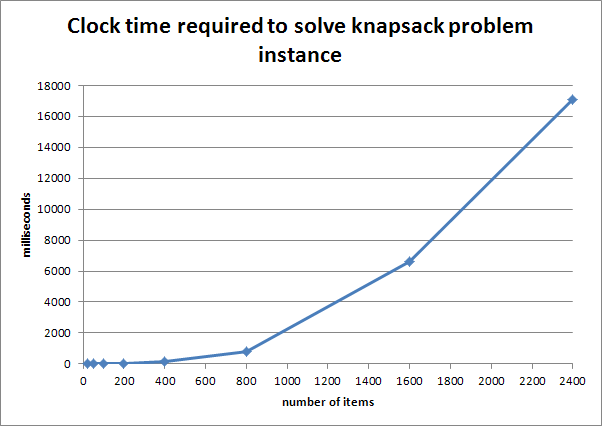
\includegraphics[scale=0.5]{pics/timing-k.eps}
\caption{Time required to solve knapsack problems of various sizes.}
\label{fig:timing-k}
\end{center}
\end{figure}


